% How every input line is classified (TickParser.parse + EventRouter). Order of the checks is the code's order.
\documentclass[tikz,border=4pt]{standalone}
\usepackage[T1]{fontenc}
\usepackage{lmodern}
\usetikzlibrary{positioning,arrows.meta,calc,shapes.geometric}
% Shared look for every diagram. \input this after \usetikzlibrary.
% Greys plus one accent, so the figures print fine in black and white.
\definecolor{accent}{HTML}{2563EB}
\definecolor{accentlight}{HTML}{DBEAFE}
\definecolor{latecol}{HTML}{B45309}
\definecolor{latelight}{HTML}{FEF3C7}
\definecolor{grey}{HTML}{6B7280}
\definecolor{greylight}{HTML}{F3F4F6}
\tikzset{
  box/.style={draw, rounded corners=2pt, align=center, minimum height=7mm, inner sep=3pt, fill=white, font=\footnotesize},
  topic/.style={box, fill=greylight, draw=grey},
  op/.style={box, draw=accent, fill=accentlight},
  ctr/.style={draw=grey, dashed, rounded corners=4pt, inner sep=3mm},
  note/.style={font=\scriptsize, text=grey, align=left},
  arr/.style={-{Latex[length=2mm]}, thick},
  shuffle/.style={arr, double, double distance=0.6pt, -{Latex[length=2.4mm]}},
  latearr/.style={arr, dashed, draw=latecol},
  lbl/.style={font=\scriptsize, fill=white, inner sep=1pt},
}

\tikzset{
  q/.style={draw=grey, diamond, aspect=2.6, inner sep=1pt, align=center, font=\scriptsize, fill=greylight},
  outk/.style={box, font=\scriptsize, minimum width=34mm, text width=34mm},
  keep/.style={outk, draw=accent, fill=accentlight},
  drop/.style={outk, draw=grey},
  yes/.style={lbl, pos=0.4, font=\tiny},
}
\begin{document}
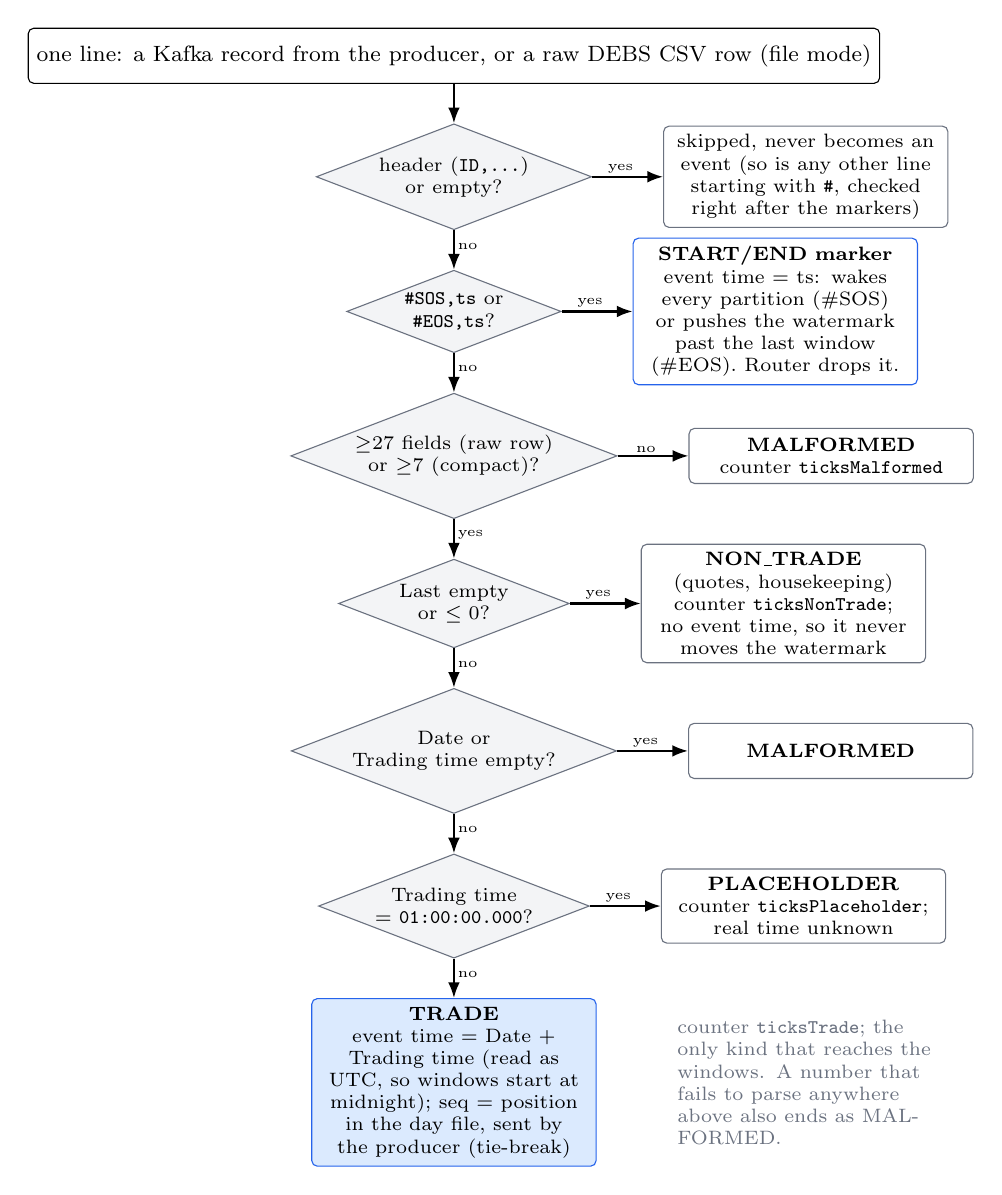
\begin{tikzpicture}[node distance=5mm and 9mm]
  \node[box] (in) {one line: a Kafka record from the producer, or a raw DEBS CSV row (file mode)};
  \node[q, below=of in] (q1) {header (\texttt{ID,\ldots})\\or empty?};
  \node[q, below=of q1] (q2) {\texttt{\#SOS,ts} or\\\texttt{\#EOS,ts}?};
  \node[q, below=of q2] (q3) {$\ge$27 fields (raw row)\\or $\ge$7 (compact)?};
  \node[q, below=of q3] (q4) {Last empty\\or $\le 0$?};
  \node[q, below=of q4] (q5) {Date or\\Trading time empty?};
  \node[q, below=of q5] (q6) {Trading time\\$=$ \texttt{01:00:00.000}?};
  \node[keep, below=of q6] (trade) {\textbf{TRADE}\\event time = Date + Trading time (read as UTC, so windows start at midnight); seq = position in the day file, sent by the producer (tie-break)};

  \node[drop, right=of q1] (skip) {skipped, never becomes an event (so is any other line starting with \texttt{\#}, checked right after the markers)};
  \node[outk, right=of q2, draw=accent] (mark) {\textbf{START/END marker}\\event time = ts: wakes every partition (\#SOS) or pushes the watermark past the last window (\#EOS). Router drops it.};
  \node[drop, right=of q3] (mal1) {\textbf{MALFORMED}\\counter \texttt{ticksMalformed}};
  \node[drop, right=of q4] (quote) {\textbf{NON\_TRADE} (quotes, housekeeping)\\counter \texttt{ticksNonTrade}; no event time, so it never moves the watermark};
  \node[drop, right=of q5] (mal2) {\textbf{MALFORMED}};
  \node[drop, right=of q6] (ph) {\textbf{PLACEHOLDER}\\counter \texttt{ticksPlaceholder}; real time unknown};
  \node[note, right=of trade, text width=34mm] {counter \texttt{ticksTrade}; the only kind that reaches the windows. A number that fails to parse anywhere above also ends as MALFORMED.};

  \draw[arr] (in) -- (q1);
  \foreach \a/\b in {q1/q2,q2/q3,q4/q5,q5/q6,q6/trade} \draw[arr] (\a) -- node[yes, right]{no} (\b);
  \draw[arr] (q3) -- node[yes, right]{yes} (q4);
  \draw[arr] (q1) -- node[yes, above]{yes} (skip);
  \draw[arr] (q2) -- node[yes, above]{yes} (mark);
  \draw[arr] (q3) -- node[yes, above]{no} (mal1);
  \draw[arr] (q4) -- node[yes, above]{yes} (quote);
  \draw[arr] (q5) -- node[yes, above]{yes} (mal2);
  \draw[arr] (q6) -- node[yes, above]{yes} (ph);
\end{tikzpicture}
\end{document}
